\section{Results}
\label{sec:results}

In this section, we present our findings based on implementing the gradient-free approach presented
earlier in Section~\ref{sec:method} for computing the active subspace, in~\ref{sub:cas}. As discussed earlier,
the uncertainty propagated from the SW parameters to thermal conductivity estimates based on NEMD
predictions is predominantly captured in the active subspace. The model output in the original space~($G$)
was approximated as $\mathcal{Y}$ in terms of active variables, $\vec\eta$ in the active subspace. A regression-fit
to $\mathcal{Y}$, $\tilde{\mathcal{Y}}$ was used as a surrogate for performing UQ. 
We verify the accuracy of the surrogate by 
estimating the relative L-2 norm of the discrepancy between NEMD-based estimates and surrogate predictions,
and performing a comparative assessment in a probabilistic sense in~\ref{sub:ver}. The verified surrogate is
used for estimating the total Sobol' indices which are shown to be consistent with the normalized activity scores,
evaluated using~\eqref{eq:ac}, in~\ref{sub:gsa}.

\subsection{Computing the active subspace}
\label{sub:cas}

The iterative procedure outlined in Algorithm~\ref{alg:free} was used to compute the active subspace. 
We began
with an initial set of 5 samples in the 7-dimensional input space. The Monte Carlo samples were drawn
from the joint probability distribution of the uncertain SW parameters, considered
to be uniformly distributed in the interval $[0.9\theta_i^\ast,1.1\theta_i^\ast]$, where $\theta_i^\ast$ are the
nominal values provided in Table~\ref{tab:sw}. 
%
\begin{table}[htbp]
\centering
\ra{1.3}
\begin{tabular}{@{}ccccccc@{}}\toprule
$A$ & $B$ & $p$ & $q$ & $\alpha$ & $\lambda$ & $\gamma$ \\
7.05 & 0.60 & 4.0 & 0.0 & 1.80 & 21.0 & 1.20 \\
\bottomrule
\end{tabular}
\caption{Nominal values of the SW potential parameters~\cite{Stillinger:1985}.}
\label{tab:sw}
\end{table}
%
Initial set of model evaluations were used to estimate the gradient vector of thermal conductivity with
individual components represent the derivative with respect to $\xi_i$ corresponding to $\theta_i$ in
the physical space. At each iteration, model evaluations at 5 new samples in the full space were 
obtained and the quantity, $\varepsilon$ was computed using~\eqref{eq:conv}.The iterative
procedure was terminated once the highest component of $\varepsilon$ was found to be smaller than
the set tolerance $\tau$ = 0.1. In this case, the process was observed to converge after 4 iterations
and required model evaluations at 25 samples, yielding $\max(\varepsilon^{(i)})$ = 0.085.
 The resulting active subspace was found to be
1-dimensional. In Figure~\ref{fig:casfig1}, we plot the components of the dominant eigenvector (left),
and the quantity, $\max(\varepsilon^{(i)})$, computed using components of the dominant eigenvector 
obtained between successive iterations, $i$ and $i-1$ (right) in~\eqref{eq:conv}.
%
\begin{figure}[htbp]
\begin{center}
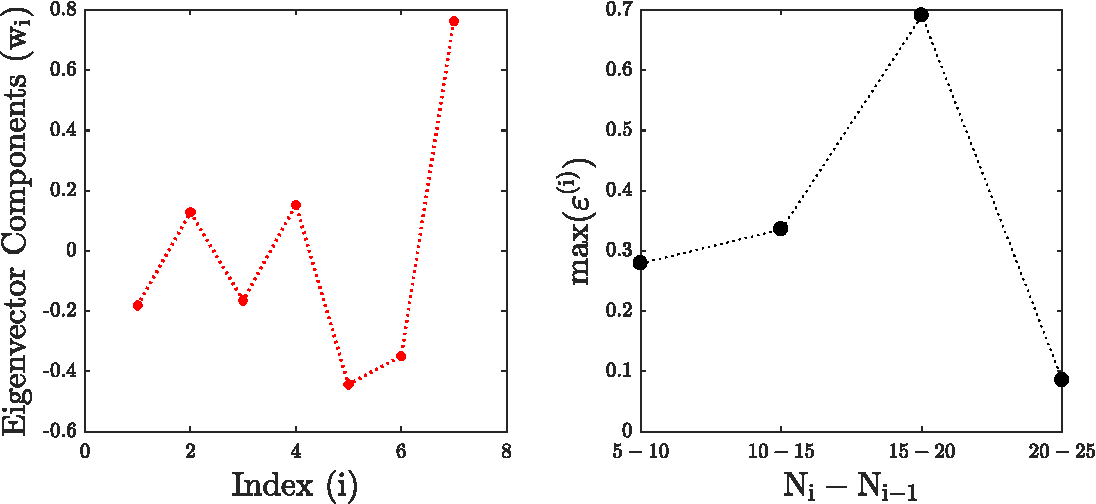
\includegraphics[width=0.8\textwidth]{./Figures/free_eigv5}
\caption{Left: Individual components of the dominant eigenvector that constitutes the 1-dimensional
active subspace. Right: A plot of $\max(\varepsilon^{(i)})$, obtained
using components of the dominant eigenvector between successive iterations.}
\label{fig:casfig1}
\end{center}
\end{figure}
%

The normalized eigenvalue spectrum is illustrated
in Figure~\ref{fig:casfig2}~(left), and the plot of $Y$ vs. $\vec\eta$, regarded as the \textit{sufficient
summary plot} (SSP) is provided in Figure~\ref{fig:casfig2}~(right). 
%
\begin{figure}[htbp]
\begin{center}
\begin{tabular}{cc}
  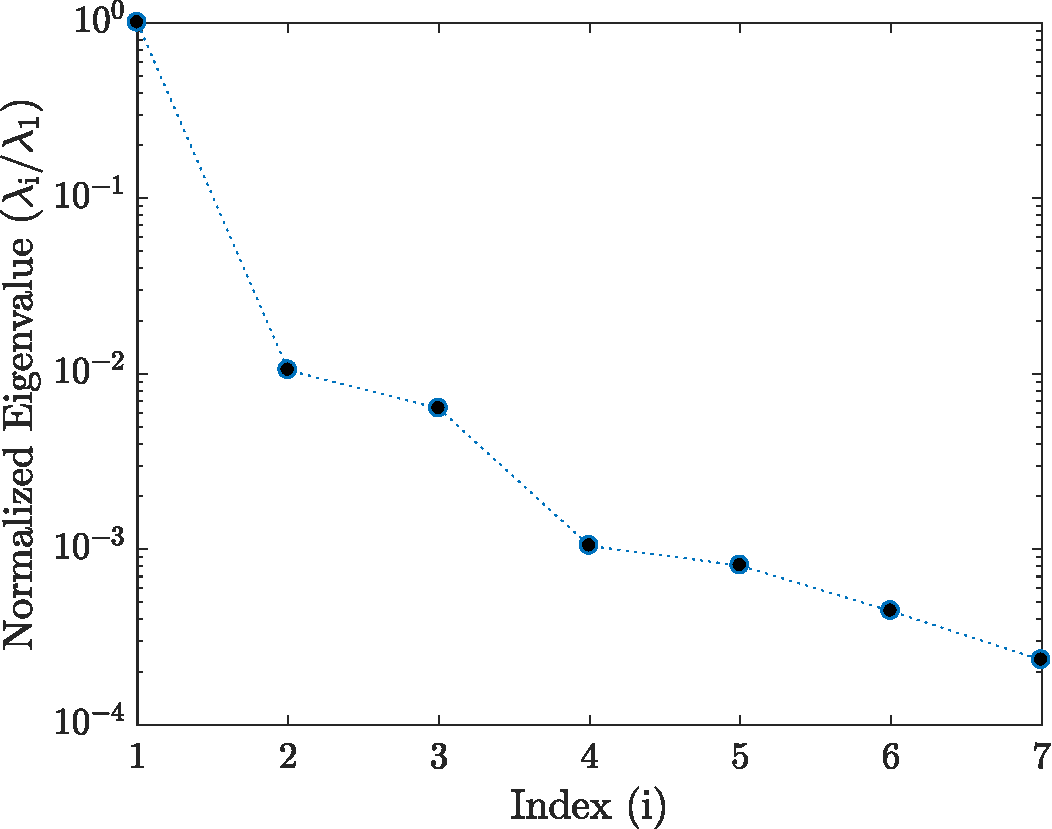
\includegraphics[width=0.42\textwidth]{./Figures/eig_spec}
  &
  \hspace{3mm}
  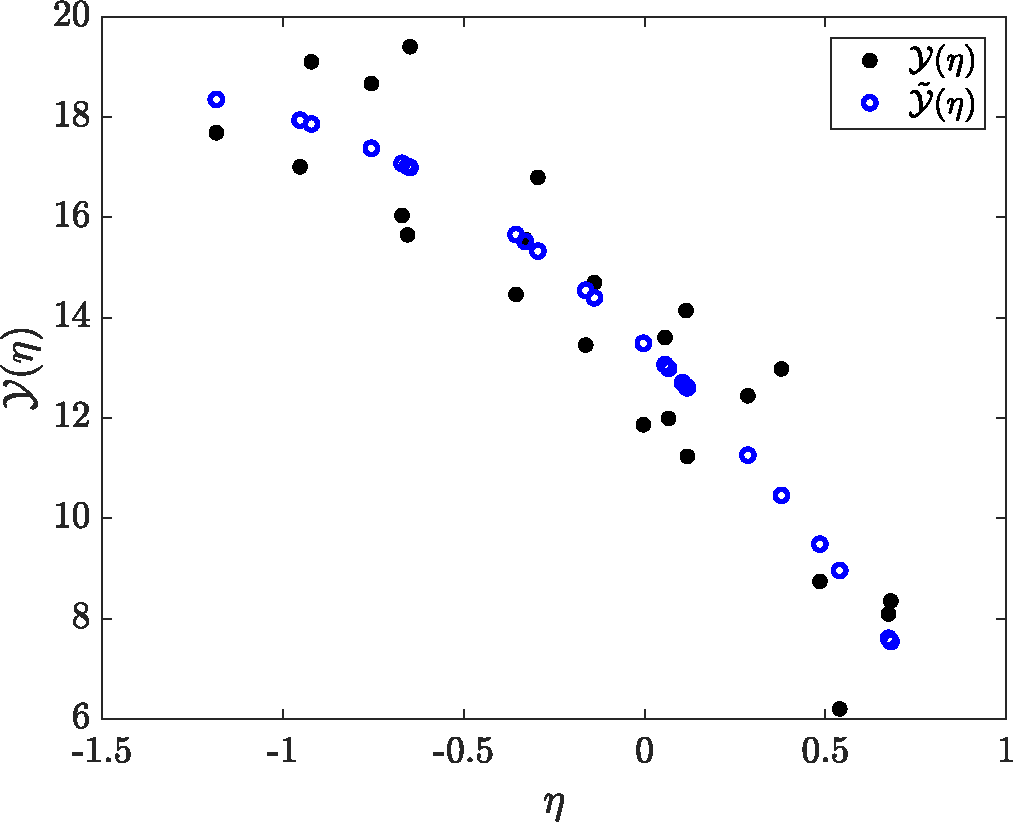
\includegraphics[width=0.4\textwidth]{./Figures/free_ssp1D}
  \end{tabular}
\caption{Left: Normalized eigenvalue spectrum of the converged matrix, $\hat{\mat{C}}$. Right: SSP
illustrating the variability of the NEMD-based thermal conductivity estimates in the 1-dimensional
active subspace.}
\label{fig:casfig2}
\end{center}
\end{figure}
%
Both plots confirm the existence of a 1-dimensional active subspace. The normalized eigenvalue specturm
indicates that the ratio of the first two eigenvalues, $\left(\frac{\lambda_1}{\lambda_2}\right)\sim\mathcal{O}(10^2)$.
Hence, the second largest eigenvalue is roughly two orders of magnitude smaller than the largest eigenvalue that
indicates a 1-dimensional subspace. Furthermore, the trends in the SSP seem to have been captured
reasonably well using a linear regression-fit which is also indicative of a 1-dimensional subspace. The linear 
fit is considered as a surrogate for $Y$ ($\tilde{Y}$). In the following section, we verify the accuracy of the
surrogate using the available set of 35 model evaluations in the 7-dimensional input space. 


\subsection{Surrogate verification}
\label{sub:ver}


\subsection{Global Sensitivity Analysis}
\label{sub:gsa}
